\documentclass[12pt, titlepage]{article}

\usepackage{fullpage}
\usepackage[round]{natbib}
\usepackage{multirow}
\usepackage{booktabs}
\usepackage{tabularx}
\usepackage{graphicx}
\usepackage{float}
\usepackage{hyperref}
\hypersetup{
    colorlinks,
    citecolor=red,
    filecolor=black,
    linkcolor=red,
    urlcolor=blue
}

%% Comments

\usepackage{color}

\newif\ifcomments\commentstrue

\ifcomments
\newcommand{\authornote}[3]{\textcolor{#1}{[#3 ---#2]}}
\newcommand{\todo}[1]{\textcolor{red}{[TODO: #1]}}
\else
\newcommand{\authornote}[3]{}
\newcommand{\todo}[1]{}
\fi

\newcommand{\wss}[1]{\authornote{blue}{SS}{#1}}
\renewcommand{\sp}[1]{\authornote{magenta}{SP}{#1}}


\newcounter{acnum}
\newcommand{\actheacnum}{AC\theacnum}
\newcommand{\acref}[1]{AC\ref{#1}}

\newcounter{ucnum}
\newcommand{\uctheucnum}{UC\theucnum}
\newcommand{\uref}[1]{UC\ref{#1}}

\newcounter{mnum}
\newcommand{\mthemnum}{M\themnum}
\newcommand{\mref}[1]{M\ref{#1}}

\newcommand{\progname}{SpecGen}

\begin{document}
\pagenumbering{gobble}

\title{CAS 741: Module Guide\\[10pt]\Large Aqueous Speciation Diagram Generator}
\author{Steven Palmer\\\texttt{palmes4}}
\date{\today}
	
\maketitle

\pagenumbering{roman}

\setcounter{secnumdepth}{0}

\section{Revision History}

\begin{table}[hp]
\caption{Revision History} \label{TblRevisionHistory}
\begin{tabularx}{\textwidth}{llX}
\toprule
\textbf{Date} & \textbf{Developer(s)} & \textbf{Change}\\
\midrule
11.02.2017 & S. Palmer & First revision of document\\
\bottomrule
\end{tabularx}
\end{table}

~\newpage

\tableofcontents

\listoftables

\listoffigures

\newpage

\pagenumbering{arabic}

\setcounter{secnumdepth}{3}

\section{Introduction}

Decomposing a system into modules is a commonly accepted approach to developing
software.  A module is a work assignment for a programmer or programming
team~\citep{ParnasEtAl1984}.  We advocate a decomposition
based on the principle of information hiding~\citep{Parnas1972a}.  This
principle supports design for change, because the ``secrets'' that each module
hides represent likely future changes.  Design for change is valuable in SC,
where modifications are frequent, especially during initial development as the
solution space is explored.  

Our design follows the rules layed out by \citet{ParnasEtAl1984}, as follows:
\begin{itemize}
\item System details that are likely to change independently should be the
  secrets of separate modules.
\item Each data structure is used in only one module.
\item Any other program that requires information stored in a module's data
  structures must obtain it by calling access programs belonging to that module.
\end{itemize}

After completing the first stage of the design, the Software Requirements
Specification (SRS), the Module Guide (MG) is developed~\citep{ParnasEtAl1984}. The MG
specifies the modular structure of the system and is intended to allow both
designers and maintainers to easily identify the parts of the software.  The
potential readers of this document are as follows:

\begin{itemize}
\item New project members: This document can be a guide for a new project member
  to easily understand the overall structure and quickly find the
  relevant modules they are searching for.
\item Maintainers: The hierarchical structure of the module guide improves the
  maintainers' understanding when they need to make changes to the system. It is
  important for a maintainer to update the relevant sections of the document
  after changes have been made.
\item Designers: Once the module guide has been written, it can be used to
  check for consistency, feasibility and flexibility. Designers can verify the
  system in various ways, such as consistency among modules, feasibility of the
  decomposition, and flexibility of the design.
\end{itemize}

The rest of the document is organized as follows. Section
\ref{SecChange} lists the anticipated and unlikely changes of the software
requirements. Section \ref{SecMH} summarizes the module decomposition that
was constructed according to the likely changes. Section \ref{SecConnection}
specifies the connections between the software requirements and the
modules. Section \ref{SecMD} gives a detailed description of the
modules. Section \ref{SecTM} includes two traceability matrices. One checks
the completeness of the design against the requirements provided in the SRS. The
other shows the relation between anticipated changes and the modules. Section
\ref{SecUse} describes the use relation between modules.

\section{Anticipated and Unlikely Changes} \label{SecChange}

This section lists possible changes to the system. According to the likeliness
of the change, the possible changes are classified into two
categories. Anticipated changes are listed in Section \ref{SecAchange}, and
unlikely changes are listed in Section \ref{SecUchange}.

\subsection{Anticipated Changes} \label{SecAchange}

Anticipated changes are the source of the information that is to be hidden
inside the modules. Ideally, changing one of the anticipated changes will only
require changing the one module that hides the associated decision. The approach
adapted here is called design for
change.

\begin{description}
\item[\refstepcounter{acnum} \actheacnum \label{acHardware}:] The specific
  hardware on which the software is running.
\item[\refstepcounter{acnum} \actheacnum \label{acEI}:] The exposed interface 
  of the library.  
\item[\refstepcounter{acnum} \actheacnum \label{acI}:] The structure of the stored
  chemical system.
\item[\refstepcounter{acnum} \actheacnum \label{acIE}:] The format of the
  input data with respect to chemical equations.  
\item[\refstepcounter{acnum} \actheacnum \label{acIS}:] The format of the
  input data with respect to chemical species.
\item[\refstepcounter{acnum} \actheacnum \label{acC}:] How the input data is 
  transformed into speciation data.
\item[\refstepcounter{acnum} \actheacnum \label{acIC}:] How the input is converted
  to a form usable by the non-linear solver.
\item[\refstepcounter{acnum} \actheacnum \label{acDG}:] How the speciation diagram
  is generated from the output data.
\item[\refstepcounter{acnum} \actheacnum \label{acNLS}:] The non-linear solver
  algorithm.
\item[\refstepcounter{acnum} \actheacnum \label{acP}:] The plotting algorithm.
\end{description}

\subsection{Unlikely Changes} \label{SecUchange}

The module design should be as general as possible. However, a general system is
more complex. Sometimes this complexity is not necessary. Fixing some design
decisions at the system architecture stage can simplify the software design. If
these decision should later need to be changed, then many parts of the design
will potentially need to be modified. Hence, it is not intended that these
decisions will be changed.

\begin{description}
\item[\refstepcounter{ucnum} \uctheucnum \label{ucIO}:] Input/Output devices
  (Input: File and/or Keyboard, Output: File, Memory, and/or Screen).
\end{description}

\section{Module Hierarchy} \label{SecMH}

This section provides an overview of the module design. Modules are summarized
in a hierarchy decomposed by secrets in Table \ref{TblMH}. The modules listed
below, which are leaves in the hierarchy tree, are the modules that will
actually be implemented.

\begin{description}
\item [\refstepcounter{mnum} \mthemnum \label{mHH}:] Hardware-Hiding Module
\item [\refstepcounter{mnum} \mthemnum \label{mEI}:] External Interface Module
\item [\refstepcounter{mnum} \mthemnum \label{mCS}:] Chemical System Module
\item [\refstepcounter{mnum} \mthemnum \label{mEP}:] Equation Parser Module
\item [\refstepcounter{mnum} \mthemnum \label{mSP}:] Species Parser Module
\item [\refstepcounter{mnum} \mthemnum \label{mC}:] Calculation Module
\item [\refstepcounter{mnum} \mthemnum \label{mIC}:] Input Conversion Module
\item [\refstepcounter{mnum} \mthemnum \label{mDG}:] Diagram Generation Module
\item [\refstepcounter{mnum} \mthemnum \label{mNLS}:] Non-linear Solver Module
\item [\refstepcounter{mnum} \mthemnum \label{mP}:] Plotting Module
\end{description}


\begin{table}[h!]
\centering
\begin{tabular}{p{0.3\textwidth} p{0.6\textwidth}}
\toprule
\textbf{Level 1} & \textbf{Level 2}\\
\midrule

{Hardware-Hiding Module} & ~ \\
\midrule

\multirow{7}{0.3\textwidth}{Behaviour-Hiding Module} & External Interface Module\\
& Chemical System Module\\
& Species Parser Module\\
& Equation Parser Module\\
& Input Conversion Module\\
& Calculation Module\\
& Diagram Generation Module\\ 
\midrule

\multirow{3}{0.3\textwidth}{Software Decision Module} & Non-linear Solver Module\\
& Plotting Module\\
\bottomrule

\end{tabular}
\caption{Module Hierarchy}
\label{TblMH}
\end{table}

\section{Connection Between Requirements and Design} \label{SecConnection}

The design of the system is intended to satisfy the requirements developed in
the SRS. In this stage, the system is decomposed into modules. The connection
between requirements and modules is listed in Table \ref{TblRT}.

\section{Module Decomposition} \label{SecMD}

Modules are decomposed according to the principle of ``information hiding''
proposed by \citet{ParnasEtAl1984}. The \emph{Secrets} field in a module
decomposition is a brief statement of the design decision hidden by the
module. The \emph{Services} field specifies \emph{what} the module will do
without documenting \emph{how} to do it. For each module, a suggestion for the
implementing software is given under the \emph{Implemented By} title. If the
entry is \emph{OS}, this means that the module is provided by the operating
system or by standard programming language libraries.  Also indicate if the
module will be implemented specifically for the software.

Only the leaf modules in the
hierarchy have to be implemented. If a dash (\emph{--}) is shown, this means
that the module is not a leaf and will not have to be implemented. Whether or
not this module is implemented depends on the programming language
selected.

\subsection{Hardware Hiding Modules (\mref{mHH})}

\begin{description}
\item[Secrets:]The data structure and algorithm used to implement the virtual
  hardware.
\item[Services:]Serves as a virtual hardware used by the rest of the
  system. This module provides the interface between the hardware and the
  software. So, the system can use it to display outputs or to accept inputs.
\item[Implemented By:] OS
\end{description}

\subsection{Behaviour-Hiding Module}

\begin{description}
\item[Secrets:]The contents of the required behaviours.
\item[Services:]Includes programs that provide externally visible behaviour of
  the system as specified in the software requirements specification (SRS)
  documents. This module serves as a communication layer between the
  hardware-hiding module and the software decision module. The programs in this
  module will need to change if there are changes in the SRS.
\item[Implemented By:] --
\end{description}

\subsubsection{External Interface Module (\mref{mEI})}

\begin{description}
\item[Secrets:]The exposed interface of the library.
\item[Services:]Provides the external interface of the library that can by used
  by programs.
\item[Implemented By:] \progname{}
\end{description}

\subsubsection{Chemical System Module (\mref{mCS})}

\begin{description}
\item[Secrets:]The structure of the stored chemical system.
\item[Services:]Provides the data structure for storing the input data.
\item[Implemented By:] \progname{}
\end{description}

\subsubsection{Equation Parser Module (\mref{mEP})}

\begin{description}
\item[Secrets:]The format of the input data with respect to chemical equations.
\item[Services:]Parses input (chemical equations) and converts to a format
  used by \mref{mCS}.
\item[Implemented By:] \progname{}
\end{description}

\subsubsection{Species Parser Module (\mref{mSP})}

\begin{description}
\item[Secrets:]The format of the input data with respect to chemical species.
\item[Services:]Parses input (chemical species) and converts to a format
  used by \mref{mCS}.
\item[Implemented By:] \progname{}
\end{description}

\subsubsection{Calculation Module (\mref{mC})}

\begin{description}
\item[Secrets:]How the input data is transformed into speciation data.
\item[Services:]Calculates equilibrium concentrations of all species over
  a pH range.
\item[Implemented By:] \progname{}
\end{description}

\subsubsection{Input Conversion Module (\mref{mIC})}

\begin{description}
\item[Secrets:]How the input is converted to a form usable by the non-linear solver.
\item[Services:]Converts input data into a format that can be passed to the non-linear solver.
\item[Implemented By:] \progname{}
\end{description}

\subsubsection{Diagram Generation Module (\mref{mDG})}

\begin{description}
\item[Secrets:]How the speciation diagram is generated from the speciation data.
\item[Services:]Generates a speciation diagram from speciation data.
\item[Implemented By:] \progname{}
\end{description}



\subsection{Software Decision Module}

\begin{description}
\item[Secrets:] The design decision based on mathematical theorems, physical
  facts, or programming considerations. The secrets of this module are
  \emph{not} described in the SRS.
\item[Services:] Includes data structure and algorithms used in the system that
  do not provide direct interaction with the user. 
  % Changes in these modules are more likely to be motivated by a desire to
  % improve performance than by externally imposed changes.
\item[Implemented By:] --
\end{description}

\subsubsection{Non-linear Solver Module (\mref{mNLS})}

\begin{description}
\item[Secrets:] The non-linear solver algorithm.
\item[Services:] Calculates a solution for a non-linear system of equations.
  % Changes in these modules are more likely to be motivated by a desire to
  % improve performance than by externally imposed changes.
\item[Implemented By:] Python
\end{description}

\subsubsection{Plotting Module (\mref{mP})}

\begin{description}
\item[Secrets:] The plotting algorithm.
\item[Services:] Produces plots (as image files). 
  % Changes in these modules are more likely to be motivated by a desire to
  % improve performance than by externally imposed changes.
\item[Implemented By:] Python
\end{description}

\newpage
\section{Traceability Matrix} \label{SecTM}

This section shows two traceability matrices: between the modules and the
requirements and between the modules and the anticipated changes.

% the table should use mref, the requirements should be named, use something
% like fref
\begin{table}[H]
\centering
\begin{tabular}{p{0.2\textwidth} p{0.6\textwidth}}
\toprule
\textbf{Req.} & \textbf{Modules}\\
\midrule
R1 & \mref{mEI}, \mref{mCS}, \mref{mEP}, \mref{mSP}\\
R2 & \mref{mCS}, \mref{mEP}, \mref{mSP}\\
R3 & \mref{mCS}\\
R4 & \mref{mEI}, \mref{mC}, \mref{mIC}, \mref{mNLS}\\
R5 & \mref{mHH}, \mref{mEI}, \mref{mDG}, \mref{mP}\\
\bottomrule
\end{tabular}
\caption{Trace Between Requirements and Modules}
\label{TblRT}
\end{table}

\begin{table}[H]
\centering
\begin{tabular}{p{0.2\textwidth} p{0.6\textwidth}}
\toprule
\textbf{AC} & \textbf{Modules}\\
\midrule
\acref{acHardware} & \mref{mHH}\\
\acref{acEI} & \mref{mEI}\\
\acref{acI} & \mref{mCS}\\
\acref{acIS} & \mref{mSP}\\
\acref{acIE} & \mref{mEP}\\
\acref{acC} & \mref{mC}\\
\acref{acIC} & \mref{mIC}\\
\acref{acDG} & \mref{mDG}\\
\acref{acNLS} & \mref{mNLS}\\
\acref{acP} & \mref{mP}\\
\bottomrule
\end{tabular}
\caption{Trace Between Anticipated Changes and Modules}
\label{TblACT}
\end{table}

\newpage
\section{Use Hierarchy Between Modules} \label{SecUse}

In this section, the uses hierarchy between modules is
provided. \citet{Parnas1978} said of two programs A and B that A {\em uses} B if
correct execution of B may be necessary for A to complete the task described in
its specification. That is, A {\em uses} B if there exist situations in which
the correct functioning of A depends upon the availability of a correct
implementation of B.  Figure \ref{FigUH} illustrates the use relation between
the modules. It can be seen that the graph is a directed acyclic graph
(DAG). Each level of the hierarchy offers a testable and usable subset of the
system, and modules in the higher level of the hierarchy are essentially simpler
because they use modules from the lower levels.

\begin{figure}[H]
\centering
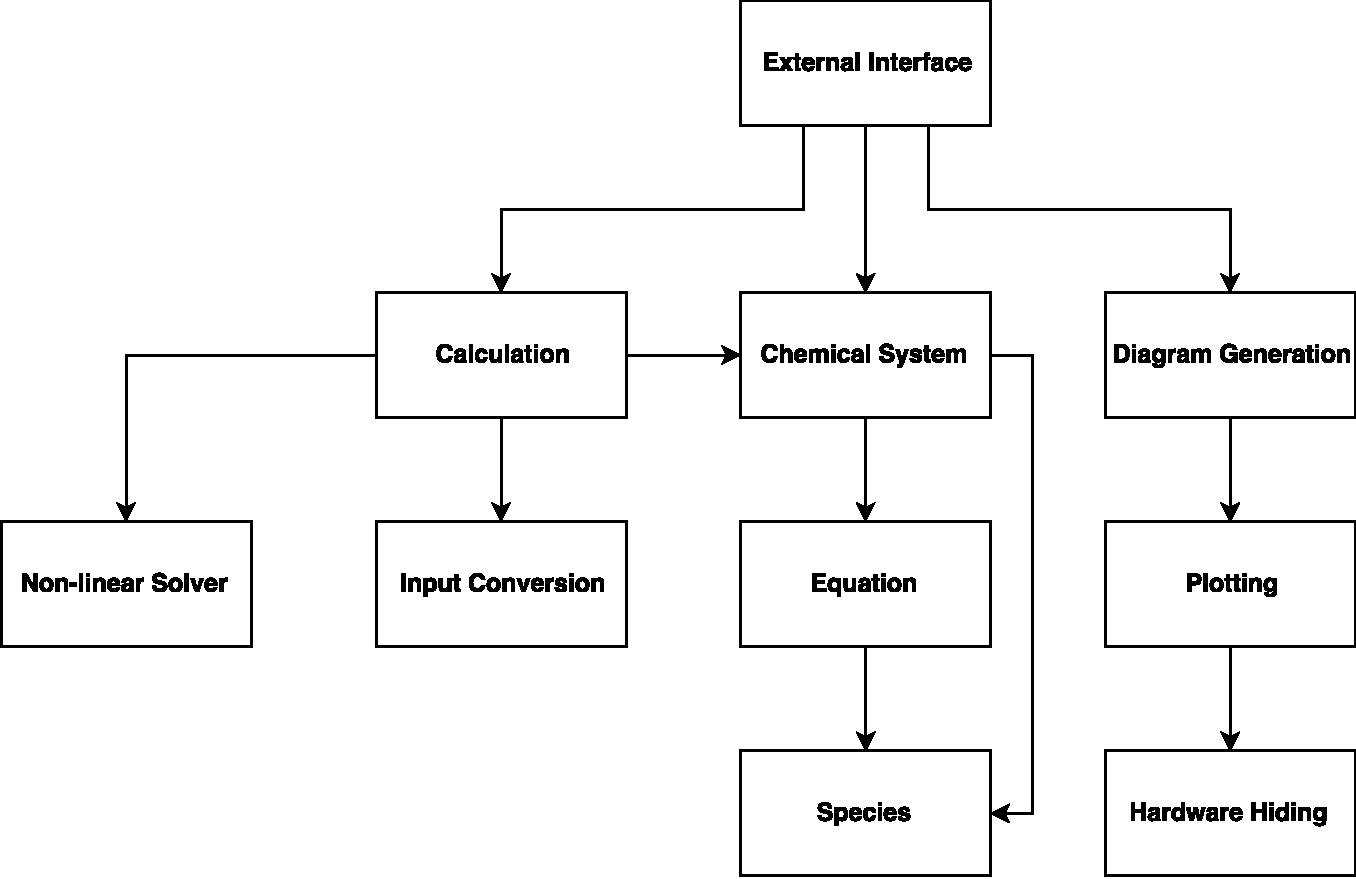
\includegraphics[width=0.8\textwidth]{UsesHierarchy.pdf}
\caption{Use hierarchy among modules}
\label{FigUH}
\end{figure}

%\section*{References}

\bibliographystyle {plainnat}
\bibliography {MG}

\end{document}